\newpage

\section{A Common Error in Generative Models}
\label{app:common_errors}
\begin{figure}[ht]
    \centering
    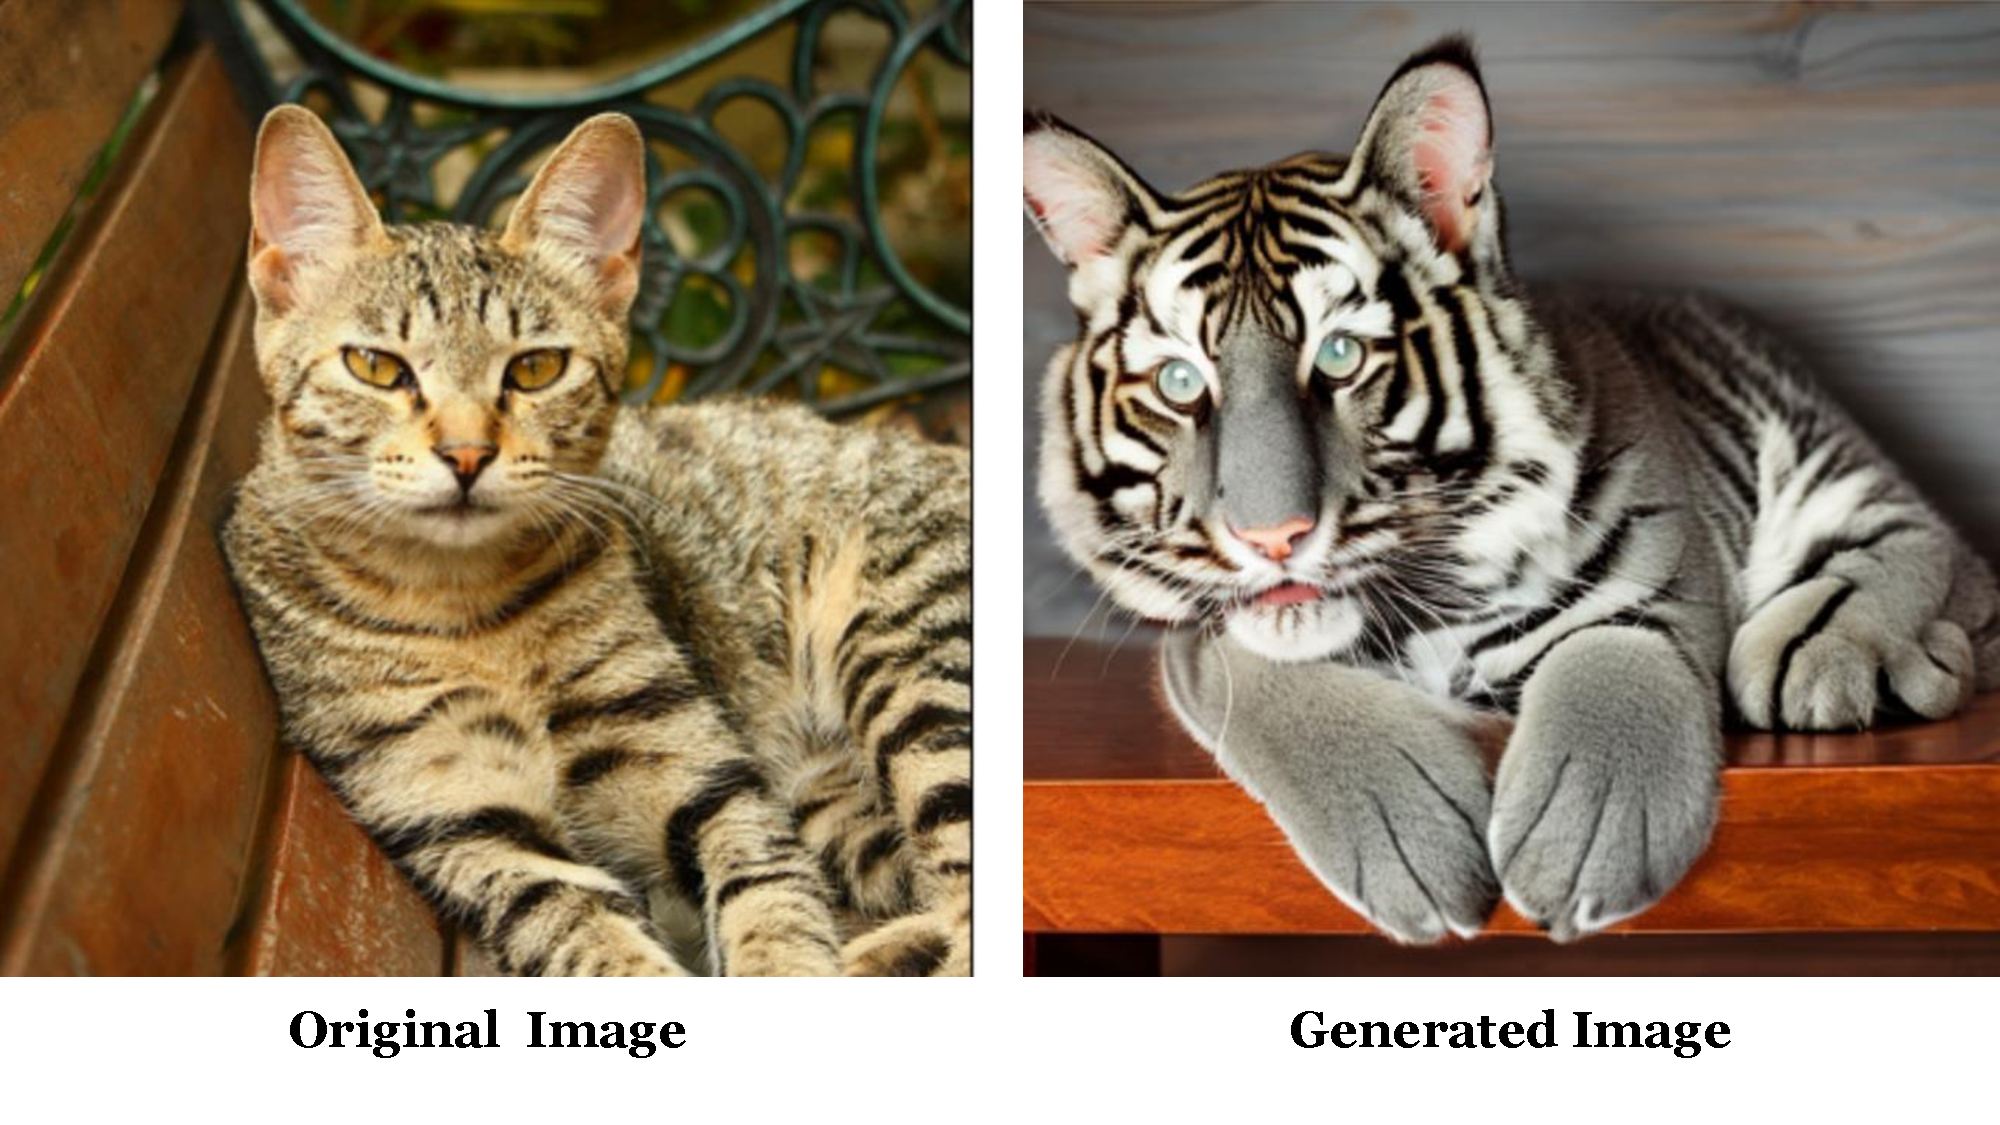
\includegraphics[width=0.8\linewidth]{figure/two_cats.pdf}
    \caption{A Common Error in Generative Models. While the original image shows “a gray tiger-striped cat,” the model incorrectly generates “a grey tiger,” illustrating semantic distortion. }
    \label{fig:common_errors}
\end{figure}

In this section, we present a common failure, attribute binding, encountered in generative models (especially for the diffusion model), where generative models misattribute visual properties to objects. Figure~\ref{fig:common_errors} compares original (left) and generated (right) images. The original depicts a gray tiger-striped cat on a wooden bench, while the generated version incorrectly shows a gray tiger instead of a cat. This issue arises because diffusion models usually rely on text encoders such as CLIP, which are known to lack the ability to capture complex linguistic structures~\citep{yuksekgonul2022and}. Consequently, the diffusion process loses awareness of the bindings between objects and their attributes, leading to mismatched visual properties. This impairs fMRI-to-image reconstruction. To address this, we introduce a neuroscience-inspired, object-centric generation approach that improves reconstruction quality.

\section{Preliminary: Diffusion Model}
\label{app:diffusion}

Diffusion models are a class of generative models that synthesize data by reversing a gradual noising process. Given a data point $ \mathbf{H}_0$ (e.g., an image), the forward process perturbs it into Gaussian noise over $T$ time steps. The model then learns the reverse process to reconstruct samples from noise. The forward process is a Markov chain defined by:
\begin{equation*}
q(\mathbf{H}_t \mid \mathbf{H}_{t-1}) = \mathcal{N}(\mathbf{H}_t; \sqrt{1 - \beta_t} \, \mathbf{H}_{t-1}, \beta_t \mathbf{I}), \quad t = 1, \ldots, T,
\end{equation*}

where \( \{ \beta_t \}_{t=1}^T \) is a predefined variance schedule. The model is trained to predict the noise \( \boldsymbol{\epsilon} \) added to the input, using a neural network \( \boldsymbol{\epsilon}_\theta \), by minimizing:

\begin{equation*}
\mathcal{L} = \mathbb{E}_{\mathbf{H}_0, \boldsymbol{\epsilon}, t} \left[ \left\| \boldsymbol{\epsilon} - \boldsymbol{\epsilon}_\theta(\mathbf{H}_t, t) \right\|^2 \right]. 
\end{equation*} 

Here, \( \mathbf{H}_t = \sqrt{\bar{\alpha}_t} \, \mathbf{H}_0 + \sqrt{1 - \bar{\alpha}_t} \, \boldsymbol{\epsilon} \), with \( \bar{\alpha}_t = \prod_{s=1}^t (1 - \beta_s) \), and \( \boldsymbol{\epsilon} \sim \mathcal{N}(0, \mathbf{I}) \). To guide the generation process with external information \( \mathbf{C} \) (e.g., a text prompt), the denoising network is extended as:
\begin{equation*}
\boldsymbol{\epsilon}_\theta(\mathbf{H}_t, t, \mathbf{C}).
\end{equation*} Then, the training objective becomes:

\begin{equation*}
\mathcal{L}_{\text{cond}} = \mathbb{E}_{\mathbf{H}_0, \boldsymbol{\epsilon}, t, \mathbf{C}} \left[ \left\| \boldsymbol{\epsilon} - \boldsymbol{\epsilon}_\theta(\mathbf{H}_t, t, \mathbf{C}) \right\|^2 \right].
\end{equation*}
This formulation is widely used in text-to-image diffusion models, where \( \mathbf{C} \) is the embedding of a textual description obtained from a pre-trained text encoder (e.g., CLIP). In practice, the condition \( \mathbf{C} \) is incorporated into the U-Net via cross-attention modules. 
%Each attention block computes:

% \begin{equation*}
% \text{CrossAttention}(\mathbf{Q}, \mathbf{K}, \mathbf{V}) = \text{softmax} \left( \frac{\mathbf{Q} \mathbf{K}^\top}{\sqrt{d}} \right) \mathbf{V},
% \end{equation*}

% where \( \mathbf{Q} = \mathbf{W}_Q \cdot \phi(\mathbf{h}_t) \) are queries from the image features, and \( \mathbf{K} = \mathbf{W}_K \cdot\varphi(\mathbf{c}) \), \( \mathbf{V} = \mathbf{W}_V \cdot \varphi(\mathbf{c}) \) are keys and values derived from the condition \( \mathbf{c} \). Here, \( \phi(\cdot) \) and \( \varphi(\cdot) \) are feature projections (e.g., linear layers, layer normalization or non-linearities depending on implementation), and $ d $ is the feature dimension. This mechanism allows the model to attend to the conditioning input \( \mathbf{c} \) at each step of generation, aligning visual outputs with semantic content.

In our work, we adopt the latent diffusion framework~\citep{rombach2022high}, where the diffusion process is applied in the latent space of a pre-trained VAE, rather than directly in pixel space. Specifically, an input image \( \mathbf{Y} \in \mathbb{R}^{H \times W \times 3} \) is first encoded by a VAE encoder into a compact latent representation \( \mathbf{Z} \in \mathbb{R}^{h \times w \times c} \):
\[
\mathbf{Z} = \text{Encoder}(\mathbf{Y}).
\]
The diffusion process is applied on \(\mathbf{Z}\), where the perturbed latent representation \(\mathbf{Z}_T\) is obtained after T steps. The reversed denoising steps then generate a denoised latent \(\hat{\mathbf{Z}}\) over T steps. The final image is reconstructed by the denoised latent:
\[
\hat{\mathbf{Y}} = \text{Decoder}(\hat{\mathbf{Z}}).
\]

This formulation greatly reduces computational cost while maintaining high-quality image generation and is particularly well-suited for conditioning on high-level semantic representations such as text or fMRI-derived embeddings.


\section{Dataset}
\label{app:dataset}

In this subsection, we provide information about the three pre-processed datasets used for the fMRI-to-image reconstruction task: NSD \citep{allen2022massive}, BOLD5000 \citep{chang2019bold5000}, and GOD \citep{horikawa2017generic}. 

\begin{itemize}
    \item \textbf{NSD} \citep{allen2022massive}: The Natural Scenes Dataset (NSD) is a large-scale public fMRI dataset capturing brain responses of human participants viewing naturalistic stimuli from COCO images \citep{lin2014microsoft}. The dataset includes scans for 30–40 hours across 30–40 separate sessions. During each session, participants viewed 750 images for 3 seconds each. Each image was presented three times across sessions, with most images unique to each subject, except for 1,000 shared images seen by all subjects. Following prior NSD reconstruction studies \citep{scotti2023reconstructing, takagi2023high}, we adopt the standardized train/test split, where the shared images serve the test set. Consequently, the training set for each subject contains 8,859 image stimuli and 24,980 fMRI trials, while the test set includes 982 image stimuli and 2,770 fMRI trials.
    
    \item \textbf{BOLD5000} \citep{chang2019bold5000}: The BOLD5000 dataset is a publicly available fMRI dataset capturing brain activity as subjects viewed a series of images. It contains 4,916 unique images, including 2,000 from the COCO dataset and 1,916 from ImageNet \citep{deng2009imagenet}. Each image was presented as a visual stimulus in individual trials. Of these, 4,803 images were shown once, while 113 images were repeated three or four times across trials, resulting in a total of 5,254 stimulus trials. We follow the standardized train/test split used in prior BOLD5000 reconstruction studies \citep{chen2023seeing, wang2024decoding}. Specifically, the training set includes trials with non-repeated image stimuli, comprising 4,803 samples, while the test set consolidate repeated image stimulus trials into 113 samples.
    
    \item \textbf{GOD} \citep{horikawa2017generic}: The Generic Object Decoding (GOD) is a public dataset developed for fMRI based decoding. It aggregates fMRI data gathered through the presentation of images from 200 representative object categories, originating from ImageNet. We follow the standardized train/test set split employed in existing GOD image reconstruction studies \citep{sun2023contrast} and get 1200 training samples and 50 test samples.The Generic Object Decoding (GOD) dataset is a publicly available fMRI dataset designed for decoding object representations. It includes fMRI data collected during the presentation of images from 200 representative object categories sourced from ImageNet. Following the standardized train/test split used in prior GOD reconstruction studies \citep{sun2023contrast}, we use 1,200 training samples and 50 test samples.
\end{itemize}








\section{Baselines}
\label{app:baseline}

In this section, we provide details about the baselines used in our experiments.


\begin{itemize}
    \item Takagi \& Nishimoto \citep{takagi2023high}: This baseline maps fMRI signals to the latent space of a pre-trained VAE within a diffusion model using linear regression, enabling image reconstruction. The method combines image latent representations with text embeddings extracted from a CLIP text encoder, both mapped from fMRI signals in higher (ventral) visual cortex regions, to improve reconstruction quality. For a fair comparison, we adapt this approach to the Diffusion 2.1 pipeline by retraining the linear regression to map fMRI signals to both the VAE latent space and the textual conditioning used in Diffusion 2.1.
            
    \item Mindvis \citep{chen2023seeing}: This baseline uses a self-supervised representation of fMRI data using masked modeling within a high-dimensional latent space in an encoder–decoder framework. The learned representation is then projected into the conditioning space of LDM by fine-tuning the model. For fair comparison, we adapt the image generator of this approach to Diffusion 2.1 by fine-tuning it with the learned projection module, following the strategy outlined by the original authors.


    
    \item Mindeye \citep{scotti2023reconstructing}: This model proposed two modules to map the fMRI signal to the CLIP image space. Specifically, the model first uses contrastive learning to align fMRI signals with image embeddings. Second, the paper trains a diffusion prior to reconstructing images from these embeddings via mapping brain activity into CLIP image space, enabling the generation of images that closely resemble the original stimuli. To adapt the method for fair comparison, we replace the Versatile Diffusion with Diffusion 2.1.
    {\color{black}
    \item MindBridge~\citep{wang2024mindbridge}: This approach unifies heterogeneous voxel dimensions using adaptive max pooling and employs a cyclic fMRI reconstruction mechanism to align neural responses across subjects in a common semantic space. To adapt the method for fair comparison, we replace the Versatile Diffusion with Diffusion 2.1.

    \item NeuralDiffuser~\citep{li2025neuraldiffuser}: This paper proposes a visual feature–guided reconstruction method that decodes multiple layers of CLIP’s visual encoder from fMRI and uses these features as gradient-based cues during the early stages of reverse diffusion, enabling bottom-up detail refinement. It further introduces momentum alignment to reduce the distribution shift between training and testing embeddings. For fair comparison, we use Diffusion 2.1 as the generative backbone.
    }
    \item Mindeye2 \citep{scotti2024mindeye2}: This method trains multiple MLPs to project fMRI signals from all subjects into a shared representation space, followed by training a diffusion prior to map these representations into the CLIP image embedding space. The final image is then reconstructed using a pre-trained SDXL~\citep{podell2023sdxl}. To adapt this method to our setting, we replace the generative backbone with Diffusion 2.1.
\end{itemize}

\section{Training Details}
\label{app:training}
In this section, we provide the training details of our model. Our model is implemented with Pytorch and trained on two NVIDIA-L40 GPUs with 48GB of memory. We use T5 as the language model to generate the object-level descriptions.  For NSD data, we train the model for 80 epochs: 60 epochs for MLP training ($E_{\text{MLP}}$) with a learning rate $\text{lr}_1 = 1 \times 10^{-5}$, followed by 20 epochs of joint training, where we continue training the MLP and fine-tune the T5 model ($E_{\text{T5}}$) using a learning rate $\text{lr}_2 = 5 \times 10^{-7}$. For BOLD5000, we set $E_{\text{mlp}}=50$,  $\text{lr}_1=1e-5$, $E_{\text{T5}}=5$, and $\text{lr}_2=1e^{10-8}$. For GOD, we set $E_{\text{mlp}}=40$, $\text{lr}_1=1e-5$, $E_{T5}=5$, and $\text{lr}_2=5e^{-9}$. For image reconstruction at inference time, we set the blending ratio $\beta=0.5$ and the denoising step as $40$ for all the datasets. We use \texttt{GPT 4o-mini} to generate the object-centric descriptions with the prompt shown in Section~\ref{app:fig:prompt}. For images that do not have a caption, we first use \texttt{GPT-4o-mini} to generate a short caption and then use our prompt to generate the object-centric description.





%\section{Additional Experiments}
{
\color{black}
\section{Case study on Object-Level Descriptions for Image Reconstruction}
\label{app:case_obj_level}

\begin{figure}[H]
    \centering
    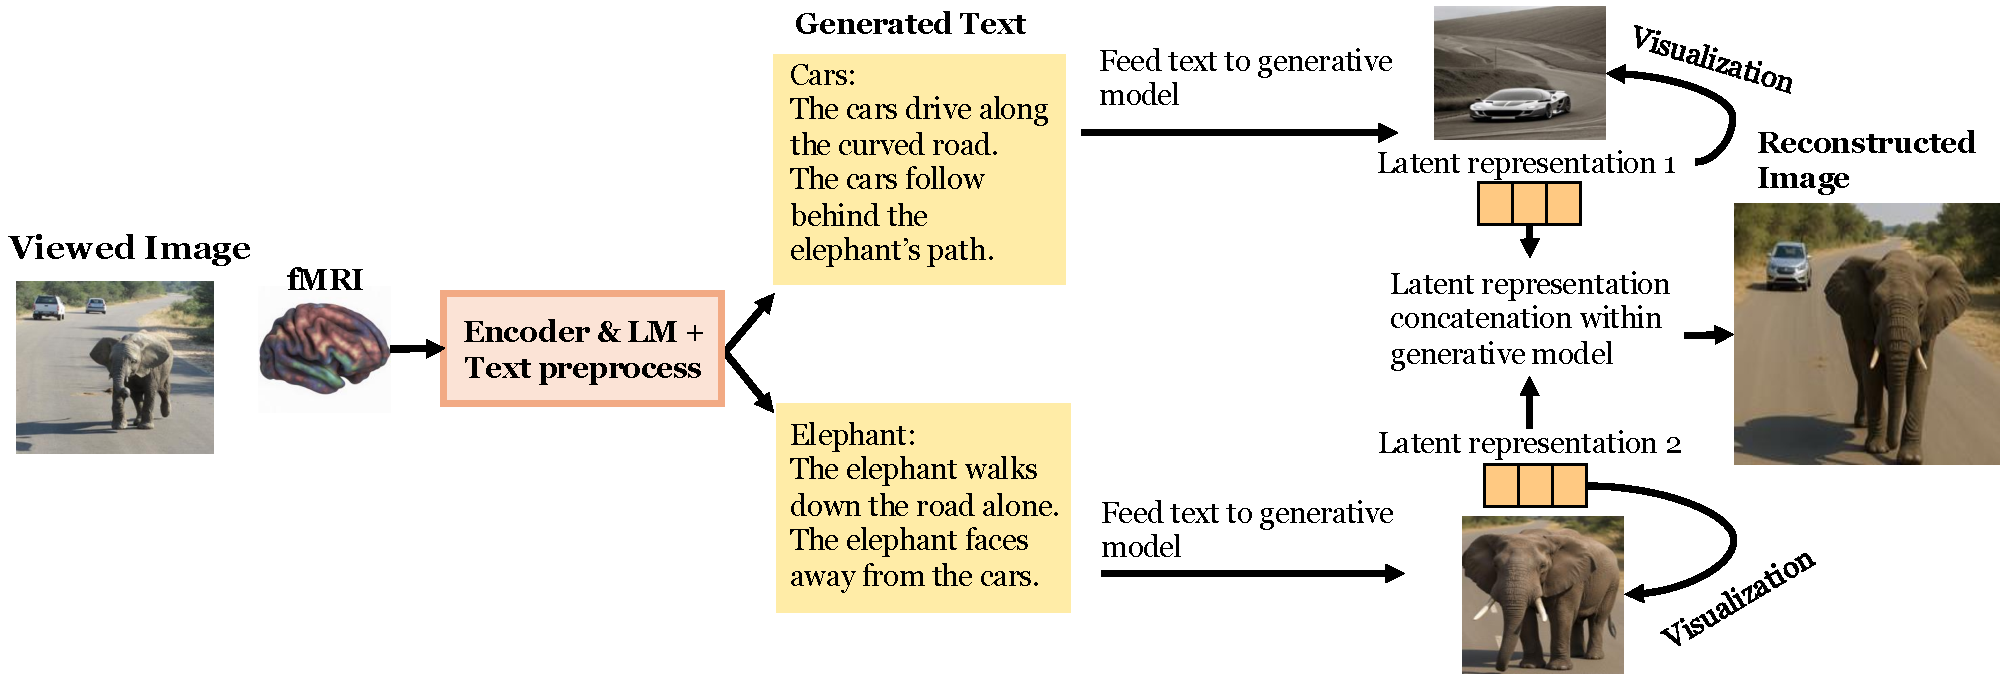
\includegraphics[width=\linewidth]{figure/obj_level.pdf}
    \caption{Reconstructed images using object-level descriptions.}
    \label{fig:obj_level}
\end{figure}

In this section, we present a case study illustrating how object-level descriptions are used during the reconstruction process, as shown in Figure~\ref{fig:obj_level}. In the given example, the generated text is segmented based on object instances: one segment describes the cars (“The cars drive along the curved road…”) and the other describes the elephant (“The elephant walks down the road alone…”). Each object description is independently fed into a diffusion-based generative model to produce object-centric latent representations. These representations are then spatially aligned and concatenated within the generative model to produce the final reconstructed image. This modular process helps mitigate common generation errors, such as attribute binding.

}






% \begin{table}[t] 
% \vspace{-0.5cm}
% \centering
% \caption{ Ablation study comparing three variants in the image reconstruction task: (1) our model with language model embeddings, (2) our model with CLIP text embeddings (Clip text), and (3) our model with image latent space from a diffusion model (LDM).The best result in each column is highlighted in \textcolor{red}{red}. $\uparrow$ indicates higher is better and $\downarrow$ indicates lower is better.}
% \resizebox{\textwidth}{!}{
% \begin{tabular}{l|ccccc|ccccc}
% \toprule
%           & \multicolumn{5}{c|}{\textbf{NSD}}   &  \multicolumn{5}{c}{\textbf{BOLD5000}} \\
%           \midrule
%           & \textbf{PixCorr} $\uparrow$ & \textbf{SSIM} $\uparrow$  & \textbf{LPIPS} $\downarrow$  & \textbf{CLIP} $\uparrow$  & \textbf{Inception V3} $\uparrow$ &  \textbf{PixCorr} $\uparrow$ & \textbf{SSIM} $\uparrow$  & \textbf{LPIPS} $\downarrow$ & \textbf{CLIP} $\uparrow$  & \textbf{Inception V3} $\uparrow$ \\ 
% \midrule
% \textbf{Ours}      & \textcolor{red}{0.3404$_{\pm 0.05}$}  & \textcolor{red}{0.4640$_{\pm 0.02}$}  & \textcolor{red}{0.5963$_{\pm 0.02}$} &     \textcolor{red}{0.9467$_{\pm 0.03}$}   & \textcolor{red}{0.9516$_{\pm 0.03}$} & \textcolor{red}{0.2315$_{\pm 0.01}$}   & \textcolor{red}{0.5341$_{\pm 0.02}$}   & \textcolor{red}{0.6198$_{\pm 0.02}$}  & \textcolor{red}{0.7720$_{\pm 0.03}$} & \textcolor{red}{0.6601$_{\pm 0.07}$}  \\
% \textbf{Clip text} & 0.3208$_{\pm 0.04}$    & 0.3725$_{\pm 0.06}$ & 0.6611$_{\pm 0.05}$ &0.9197$_{\pm 0.02}$  &  0.9011$_{\pm 0.04}$ & 0.2000$_{\pm 0.06}$   & 0.4885$_{\pm 0.06}$ & 0.6520$_{\pm 0.04}$ & 0.7265$_{\pm 0.04}$ & 0.6199$_{\pm 0.04}$     \\
% \textbf{LDM}   & 0.2090$_{\pm 0.07}$  & 0.3727$_{\pm 0.07}$ & 0.7502$_{\pm 0.04}$ & 0.8602 $_{\pm 0.06}$ & 0.8925 $_{\pm 0.05}$ & 0.1622$_{\pm 0.03}$  &0.4300$_{\pm 0.02}$  & 0.7894$_{\pm 0.08}$   & 0.7025$_{\pm 0.08}$ & 0.5590 $_{\pm 0.05}$ \\

% \bottomrule
% \end{tabular}
% }
% \vspace{0.1cm}
% \label{tb:main}
% \end{table}




\section{Reconstruction performance across different latent spaces} 

We report the ablation studies to justify our choice of text as the latent space on BOLD5000 and GOD. As shown in Table~\ref{tb:app_abl_space}, aligning fMRI signals to the language model text space (our method) consistently outperforms alignment to the other two spaces across all metrics. This supports our core contribution: textual representations alone are sufficient to capture both high-level semantic and low-level visual information, and text space provides a more brain-aligned and effective intermediate representation for fMRI-to-image reconstruction.



\begin{table}[t] 
\vspace{-0.5cm}
\centering
\caption{Reconstruction performance across three latent spaces. The best result in each column is highlighted in \textcolor{red}{red}. $\uparrow$ indicates higher is better and $\downarrow$ indicates lower is better.}
\resizebox{\textwidth}{!}{
\begin{tabular}{lccccc}
\toprule
          
          & \textbf{PixCorr} $\uparrow$ & \textbf{SSIM} $\uparrow$  & \textbf{LPIPS} $\downarrow$  & \textbf{CLIP} $\uparrow$  & \textbf{Inception V3} $\uparrow$  \\ 

%           \multicolumn{5}{l}{\textbf{NSD}} &   \\
% \midrule
% \textbf{Ours}      & \textcolor{red}{0.3404$_{\pm 0.05}$}  & \textcolor{red}{0.4640$_{\pm 0.02}$}  & \textcolor{red}{0.5963$_{\pm 0.02}$} &     \textcolor{red}{0.9467$_{\pm 0.03}$}   & \textcolor{red}{0.9516$_{\pm 0.03}$}  \\
% \textbf{Clip text} & 0.3208$_{\pm 0.04}$    & 0.3725$_{\pm 0.06}$ & 0.6611$_{\pm 0.05}$ &0.9197$_{\pm 0.02}$  &  0.9011$_{\pm 0.04}$  \\
% \textbf{LDM}   & 0.2090$_{\pm 0.07}$  & 0.3727$_{\pm 0.07}$ & 0.7502$_{\pm 0.04}$ & 0.8602 $_{\pm 0.06}$ & 0.8925 $_{\pm 0.05}$ 
% \\ 
          \midrule

\multicolumn{5}{l}{\textbf{BOLD5000}} &   \\

\midrule

\textbf{Ours} &\textcolor{red}{0.2315$_{\pm 0.01}$}   & \textcolor{red}{0.5341$_{\pm 0.02}$}   & \textcolor{red}{0.6198$_{\pm 0.02}$}  & \textcolor{red}{0.7720$_{\pm 0.03}$} & \textcolor{red}{0.6601$_{\pm 0.07}$} \\

\textbf{Clip text} & 0.2000$_{\pm 0.06}$   & 0.4885$_{\pm 0.06}$ & 0.6520$_{\pm 0.04}$ & 0.7265$_{\pm 0.04}$ & 0.6199$_{\pm 0.04}$ \\

\textbf{LDM} & 0.1622$_{\pm 0.03}$  &0.4300$_{\pm 0.02}$  & 0.7894$_{\pm 0.08}$   & 0.7025$_{\pm 0.08}$ & 0.5590 $_{\pm 0.05}$\\

\midrule
\multicolumn{5}{l}{\textbf{GOD}} &   \\
\midrule



\textbf{Ours} & \textcolor{red}{0.2571 $_{\pm 0.01}$}   & \textcolor{red}{0.5200 $_{\pm 0.02}$} & \textcolor{red}{0.6213 $_{\pm 0.01}$} & \textcolor{red}{0.8567 $_{\pm 0.05}$} & \textcolor{red}{0.8428 $_{\pm 0.06}$} \\

\textbf{Clip text} & 0.2200 $_{\pm 0.05}$  & 0.4682 $_{\pm 0.04}$& 0.6827 $_{\pm 0.04}$ & 0.8120 $_{\pm 0.05}$ & 0.7602 $_{\pm 0.04}$ \\


\textbf{LDM} & 0.1900$_{\pm 0.02}$  & 0.3999$_{\pm 0.07}$  & 0.7100$_{\pm 0.02}$   & 0.7099$_{\pm 0.01}$ & 0.7484 $_{\pm 0.03}$ \\
\bottomrule

\end{tabular}
\label{tb:app_abl_space}

}
\vspace{0.1cm}
\end{table}









\section{Analysis on the number of objects in our framework}
\label{app_mlp}
In our framework, we fix the number of objects per image to two and assign a separate MLP to each. We learn to assign each object a location label from a predefined set of spatial positions (e.g., left/right or top/bottom). This fixed assignment of each object to a dedicated MLP, along with the predefined spatial labeling scheme, is used consistently during both training and inference. At inference time, each MLP independently encodes fMRI signals for one object, and the language model generates a structured description for each. These descriptions are then passed to the object-centric diffusion model, which generates object images independently and places them into their corresponding spatial positions to form the final image.



\begin{table}[]
\caption{Comparison of the number of objects in our framework. Results are reported using PixCorr, SSIM, LPIPS, CLIP, and Inception V3 metrics. The best result in each column is highlighted in \textcolor{red}{red}. $\uparrow$ indicates higher is better and $\downarrow$ indicates lower is better.}
\resizebox{\textwidth}{!}{

\begin{tabular}{lccccc}
\toprule
          & PixCorr $\uparrow$      & SSIM $\uparrow$         & LPIPS $\downarrow$      & CLIP $\uparrow$         & Inception V3 $\uparrow$ \\
\midrule
Ours (Two Objs) & \textcolor{red}{0.3404 $_{\pm 0.05}$} & \textcolor{red}{0.464 $_{\pm 0.02}$} & \textcolor{red}{0.5943 $_{\pm 0.02}$ }& \textcolor{red}{0.9467 $_{\pm 0.03}$} & \textcolor{red}{0.9516 $_{\pm 0.03}$} \\
One Obj   & 0.3355 $_{\pm 0.05}$ & 0.4532 $_{\pm 0.04}$ & 0.6014 $_{\pm 0.04}$ & 0.9344 $_{\pm 0.02}$ & 0.9342 $_{\pm 0.01}$ \\
Four Objs & 0.3202 $_{\pm 0.03}$ & 0.4469 $_{\pm 0.04}$ & 0.6284 $_{\pm 0.02}$ & 0.9400 $_{\pm 0.05}$ & 0.9322 $_{\pm 0.05}$ \\
\bottomrule
\end{tabular}
\label{tb:mlps}

}
\end{table}


\textcolor{black}{
We conduct an experiment to determine the optimal number of objects (MLPs) in our framework, and the results on the NSD dataset are reported in Table~\ref{tb:mlps}. The results show that setting the number of objects per image to two yields the best performance. We further present case studies for setting $m=2$ and $m=4$ in Figures~\ref{fig:m2_4_succ} and~\ref{fig:m2_4}, respectively. We observe that for more complex images (i.e., those containing four objects), setting 
$m=2$ encourages the VLM to describe the first object as a group of similar instances, rather than generating isolated descriptions for each object. As shown in Figure~\ref{fig:m2_4_succ}, the individual players are grouped and described as “three players.” In contrast, setting $m=4$ prompts the VLM to generate object-level descriptions (e.g., generating one description per player, as shown in Figure~\ref{fig:m2_4}), leading the generative model to produce distinct latent representations for each object. These representations are then concatenated by spatial location and passed to the pre-trained diffusion model. However, when too many object-level features are introduced, the diffusion model tends to omit objects during the denoising process \cite{liu2024correcting, wang2023imagen}, resulting in incomplete reconstructions—for example, with one of three players missing in the final output (Figure~\ref{fig:m2_4_succ}).
}






\begin{figure}[ht]
    \centering
    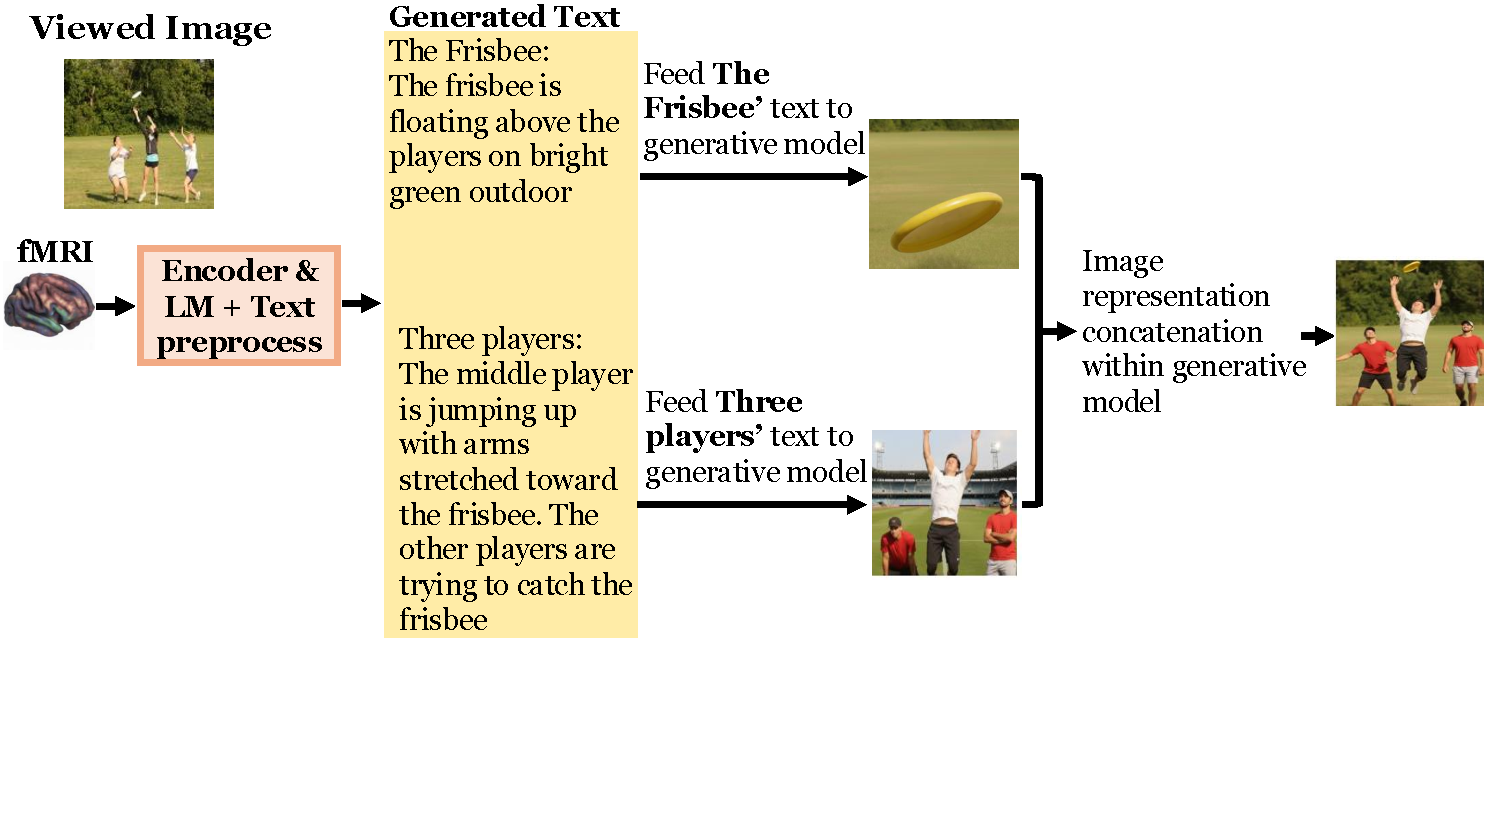
\includegraphics[width=\linewidth]{figure/m_2_4_succ.pdf}
    \vspace{-2cm}
    \caption{Reconstructed images using two objects.}
    \label{fig:m2_4_succ}
\end{figure}


\begin{figure}[ht]
    \centering
    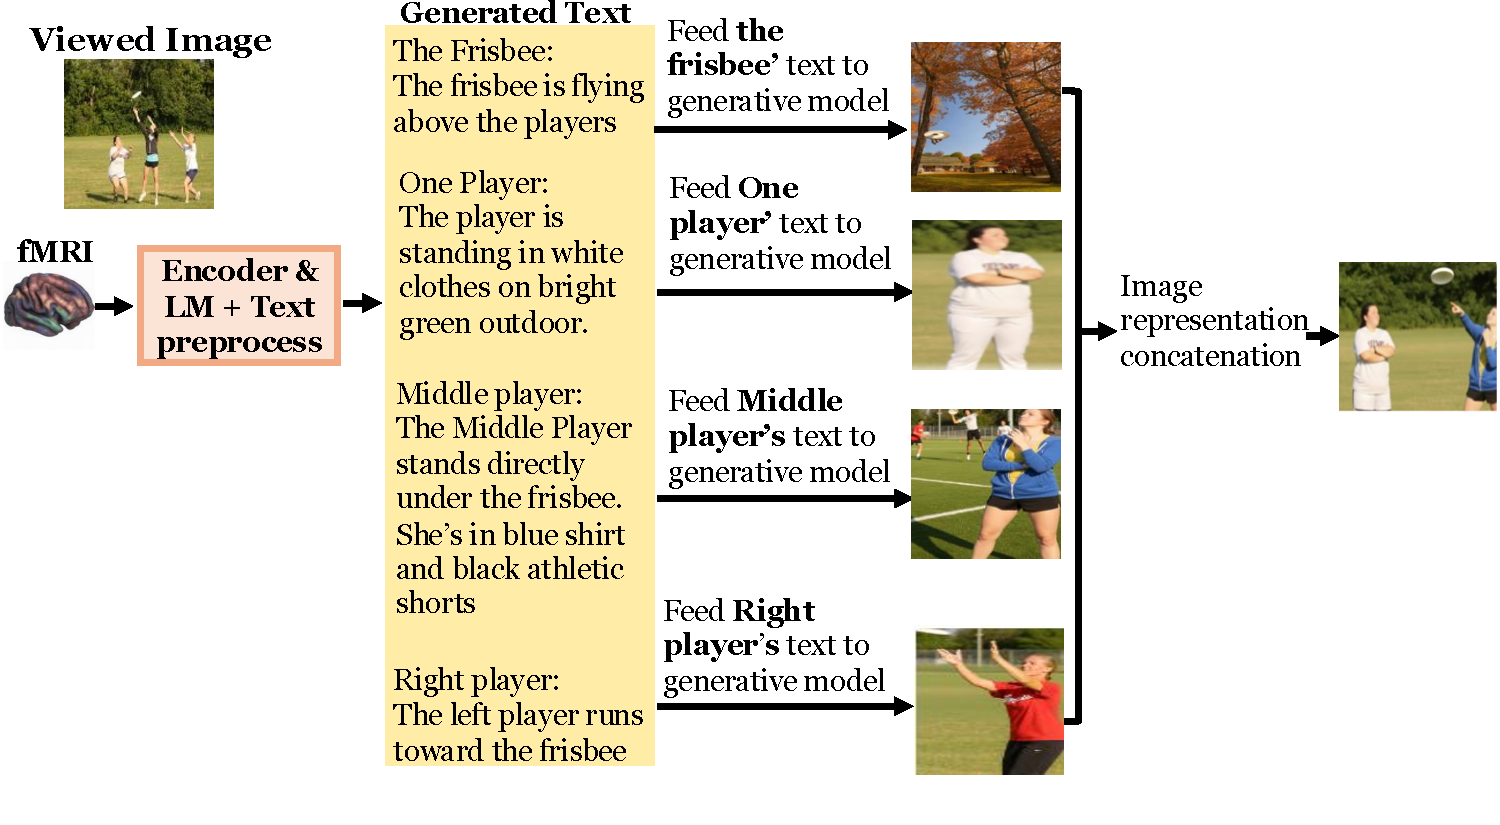
\includegraphics[width=\linewidth]{figure/m_2_4.pdf}
    \vspace{-1cm}
    \caption{Reconstructed images using four objects.}
    \label{fig:m2_4}
\end{figure}

% This choice is also supported by neuroscientific findings suggesting that, although the number of objects in an image is inherently uncertain, human attention and memory are limited to only a few of the objects. Both empirical experiments~\cite{alvarez2007many} and neural evidence~\cite{cowan2001magical, todd2004capacity} show that humans can attend to only 3–4 simple objects (e.g., a circle on a white background) at a time. For complex objects (e.g., those with intricate color patterns), this capacity drops to around 2 due to the increased cognitive load per item~\cite{xu2006dissociable}. 


% This cognitive bottleneck limits the amount of information that can be decoded from fMRI signals. As a result, increasing the number of $m$ does not necessarily enhance the level of detail in the reconstructed image and may even lead to less reliable reconstructions—for example, by hallucinating non-existent objects. Therefore, we choose to use $m=2$, as it empirically yields the best performance.



\section{Attribute/relationship Optimization Details}
\label{app:attr_opt}

The detailed algorithm used to solve the prompt optimization problem in~\Cref{eq:opt_obj} is provided in Algorithm~\ref{alg:attr_opt}.
In our experiments, we adopt the scoring function $\mathcal{S}(\mathbf{Y}_1,\mathbf{Y}_2) = 1 - \text{LPIPS}(\mathbf{Y}_1,\mathbf{Y}_2)$. The CKA threshold $\beta$ is initialized to the minimum CKA score among the initial candidates.
We set $\varepsilon=0.5,k_1=8,k_2=2$ and search for $T=40$ rounds. We randomly sampled 667 images from the training set of \textbf{NSD}~\citep{allen2022massive} for prompt optimization. While this subset is used for efficiency, our method is applicable to the full training set and generalizes to other settings. We use \texttt{GPT-4o-mini} as the VLM and the LLM that generates new keywords. We use CLIP-text \citep{radford2021learning} as $\text{LM}_{\text{ENC}}$, and Stable Diffusion 2.1 \citep{pernias2023wurstchen, rombach2022high} as the diffusion model.

\begin{algorithm}[ht]
   \caption{$\varepsilon$-Greedy Prompt Optimization}
   \label{alg:attr_opt}
\begin{algorithmic}
   \STATE \textbf{Input:} Training set $\mathcal{X}^{\text{train}}, \mathcal{Y}^{\text{train}}$; Initial keyword set $\mathcal{A}$; Search rounds $T$; Parameters $\varepsilon, k_1, k_2$
   \STATE \textbf{Initialize:} Threshold $\beta \leftarrow \min_{a \in \mathcal{A}} \text{CKA}\left(\mathbf{X}, \mathbf{K}^a\right)$
   \FOR{$t = 1$ to $T$}
       \STATE \textbf{Filter:} $\mathcal{A} \leftarrow \{a \in \mathcal{A} \mid \text{CKA}\left(\mathbf{X}, \mathbf{K}^a\right) > \beta\}$
       \STATE \textbf{Sort:} Rank $a\in\mathcal{A}$ in descending order by $\sum_{i=1}^N\mathcal{S}\left(\mathbf{Y}_i,\text{Diff}(\text{VLM}(\mathbf{Y}_i,\mathcal{P}(a)))\right)$
       \IF{\texttt{random()} $< \varepsilon$}
           \STATE \textbf{Sample:} $\mathcal{S} \leftarrow \text{RandomSample}(\mathcal{A}, k_1)$ \hfill\% Randomly sample $k_1$ keywords from $\mathcal{A}$
       \ELSE
           \STATE \textbf{Select:} $\mathcal{S} \leftarrow \text{Top}(\mathcal{A}, k_1)$ \hfill\% Select top-$k_1$ keywords from $\mathcal{A}$
       \ENDIF
       \STATE \textbf{Generate:} Use LLM to synthesize $k_2$ new keywords $\mathcal{A}_{\text{new}}$ based on $\mathcal{S}$
       \STATE \textbf{Update:} $\mathcal{A} \leftarrow \mathcal{A} \cup \mathcal{A}_{\text{new}}$
   \ENDFOR
   \STATE \textbf{Output:} $\arg\max_{a \in \mathcal{A}} \sum_{i=1}^N\mathcal{S}\left(\mathbf{Y}_i,\text{Diff}(\text{VLM}(\mathbf{Y}_i,\mathcal{P}(a)))\right)$
\end{algorithmic}
\end{algorithm}

The search is initialized with six widely-used keywords describing object attributes and relationships: Semantic Relationship~\citep{johnson2015image}, Positional Relationship~\citep{lu2016visual,haldekar2017identifying}, Functional Attributes~\citep{zhu2015understanding}, Action Attributes~\citep{lu2016visual}, Visual Attributes~\citep{farhadi2009describing}, and Part–Whole Relationship~\citep{lu2016visual}. For each type, we use \texttt{GPT-4o} to generate four synonymous keywords, resulting in an initial pool of 24 candidate keywords. Figure~\ref{fig:keywords} reports the LPIPS scores of all initial and subsequently discovered keywords.

{\color{black}
\section{Keyword Search with Different Initial Sets}
\label{app:new_keyword_search}
To further demonstrate the effectiveness of our attribute/relationship search module, we conduct an additional experiment where we excluded spatial-related keywords from the initial keyword set. We then evaluated whether our search procedure could still find spatially relevant terms. As shown in Table~\ref{tab:keyword_evolution_app}, the module successfully identifies spatial keywords under this constraint, demonstrating the robustness and effectiveness of our search process.
}

\begin{table}[h]
{
\color{black}
\caption{Top-5 discovered keywords across search rounds.}
\label{tab:keyword_evolution_app}
\setlength{\tabcolsep}{6pt}
\footnotesize
\begin{tabular}{lcccc}
\toprule
\textbf{Rank} & \textbf{Round 0} & \textbf{Round 10} & \textbf{Round 20} & \textbf{Round 30} \\
\midrule
\#1 & Textural Attribute    & Spatial Relationship & Spatial Arrangement & Spatial Arrangement \\
\#2 & Conceptual Linkage    & Textural Attribute   & Proximity Dynamics  & Proximity Relation  \\
\#3 & Action Interaction    & Visual Harmony       & Spatial Relationship & Proximity Dynamics \\
\#4 & Chromatic Feature     & Emotional Resonance  & Color Arrangement   & Spatial Relationship \\
\#5 & Attribute Description & Conceptual Linkage   & Hue Contrast        & Color Arrangement \\
\bottomrule
\end{tabular}
}
\end{table}


\section{Prompts used by \modelname}
% The prompt used by the \texttt{GPT-4o-mini} is shown below:
\begin{figure}[H]
    \centering
    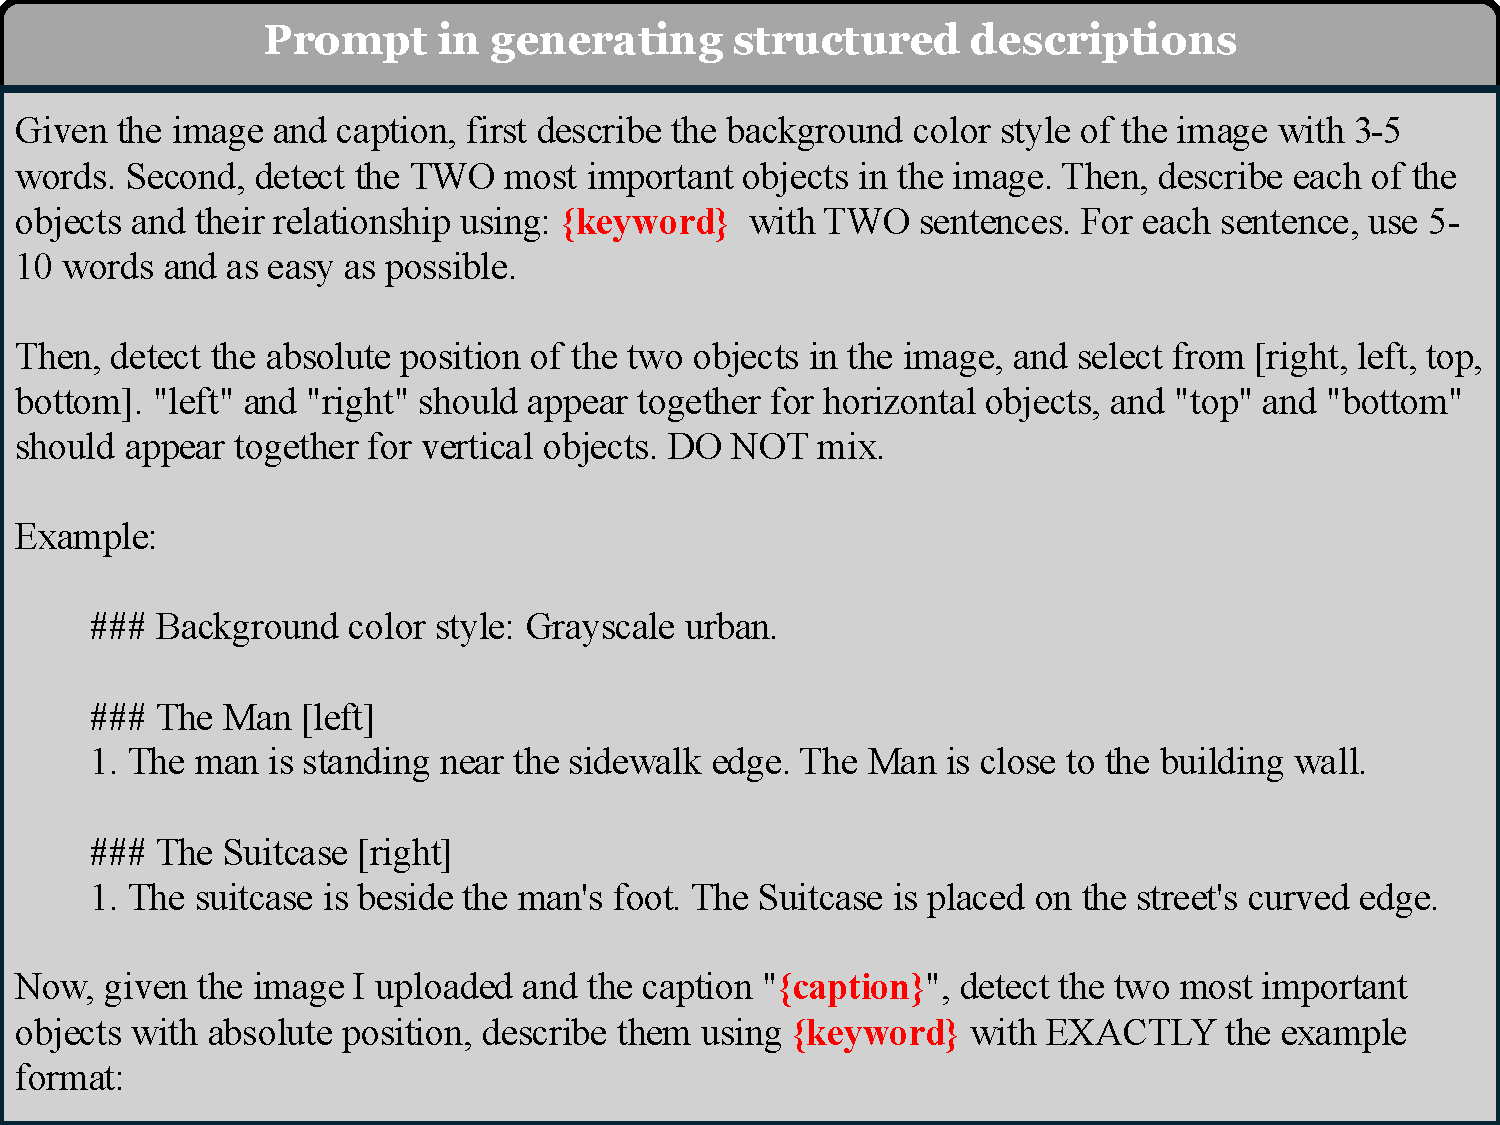
\includegraphics[width=\linewidth]{figure/prompt.pdf}
    \label{app:fig:prompt}
    \centering
    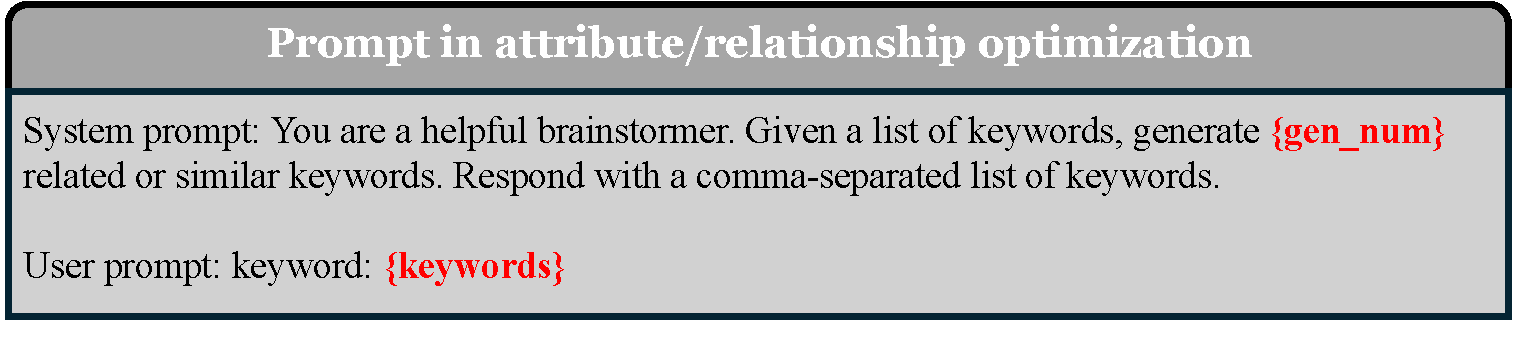
\includegraphics[width=\linewidth]{figure/prompt_opt.pdf}
    \label{app:fig:prompt_opt}
\end{figure}

\begin{figure}[H]
    \centering
    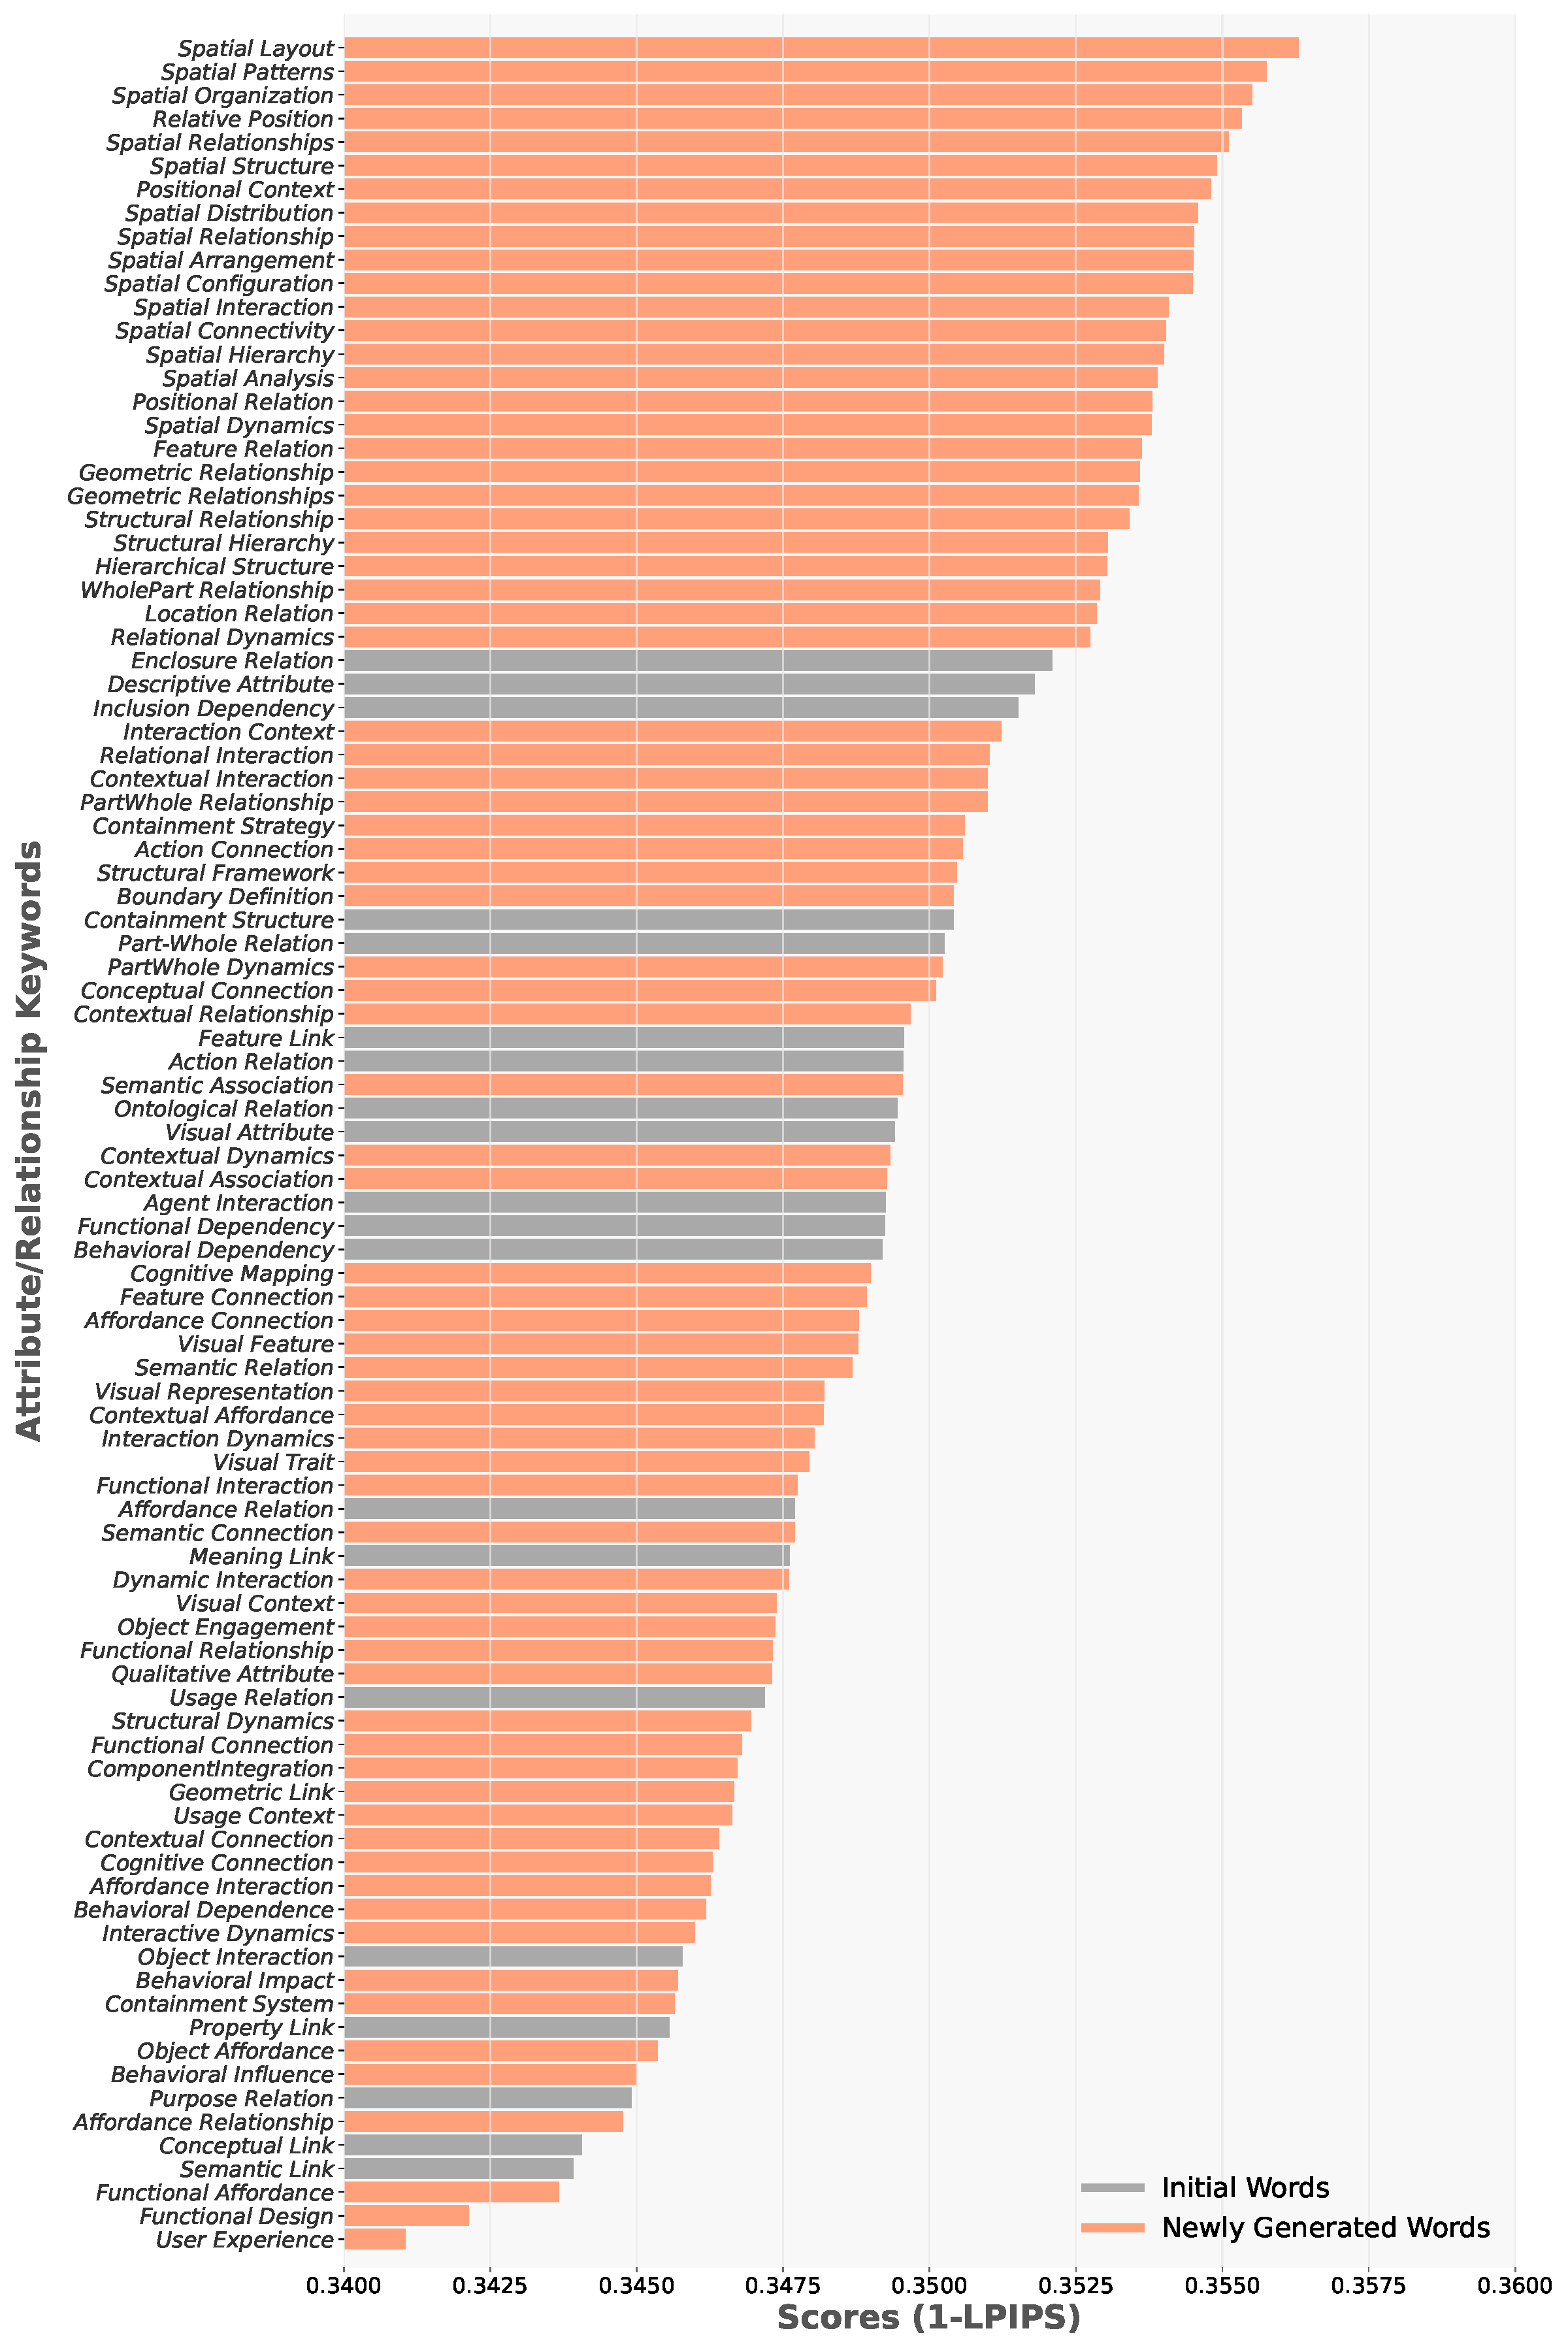
\includegraphics[width=\linewidth]{figure/keywords_bar.pdf}
    \caption{Scores of all keywords during the prompt search. Among the top-10 keywords, the most frequent keyword is 'spatial'.}
    \label{fig:keywords}
\end{figure}

\section{The Use of Large Language Models (LLMs)
}
We declare that Large Language Models (LLMs) were confined to peripheral tasks and had no influence on the methodology, results interpretation, or theoretical insights of this work. Specifically, they were used for (i) generating training datasets required for our experiments and (ii) grammar correction and minor word-level refinements. All language edits were carefully reviewed by the authors to ensure that no hallucinations were introduced and that the text faithfully reflects the original intent. The technical development, experimental design, analysis, and conclusions presented here are entirely the work of the authors.








% \section{\textcolor{red}{Rebuttal}}

% no rebuttal section, add to conres section

% \subsection{\textcolor{red}{Case study on different numbers of objects}}



% \section{Prompts Used in \modelname}
% In this subsection, we present the prompts used for generating object-centric descriptions and for attribute optimization.





% \section{Limitations}
% \label{app:limitation}
% Our approach to fMRI-to-image reconstruction is grounded in the use of generative models and relies on the finding that language model text space provides a suitable bridge for the brain’s amodal semantic representation system. However, whether this text space truly reflects the structure of human conceptual representations remains an open question and needs further investigation from neuroscience. Additionally, our framework currently focuses on fMRI data, which provides relatively coarse spatial and temporal resolution. Extending the method to incorporate other neural recording modalities—such as magnetoencephalography (MEG) or electroencephalography (EEG)—could enable more temporally precise decoding and broaden the applicability of brain-to-image reconstruction systems.



% \section{Broader Impacts}
% \label{app:broader_impact}
% This work advances the field of brain-computer interfaces by proposing a neuroscience-inspired framework for reconstructing images from fMRI data using generative diffusion models. By bridging neural activity and visual generation through object-centric language representations, our approach offers potential applications in cognitive neuroscience, assistive communication technologies for individuals with paralysis, and neural decoding research. We do not see negative societal consequences arising from our work.


